% Created by tikzDevice version 0.9 on 2015-11-20 12:13:52
% !TEX encoding = UTF-8 Unicode
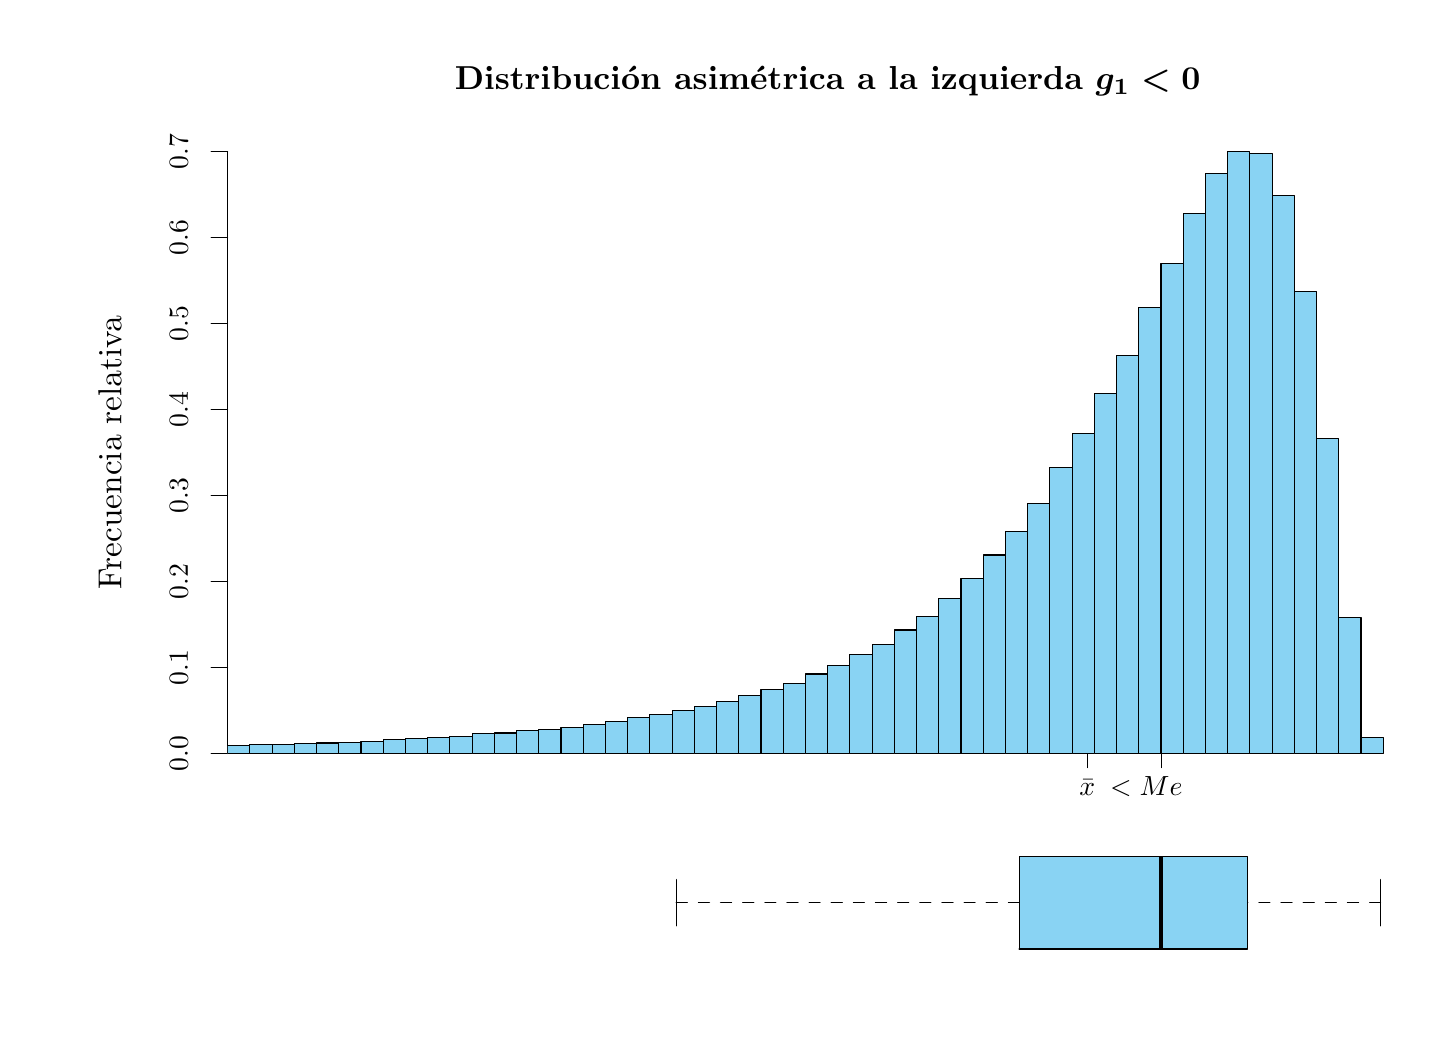
\begin{tikzpicture}[x=1pt,y=1pt]
\definecolor{fillColor}{RGB}{255,255,255}
\path[use as bounding box,fill=fillColor,fill opacity=0.00] (0,0) rectangle (505.89,361.35);
\begin{scope}
\path[clip] (  0.00, 90.34) rectangle (505.89,361.35);
\definecolor{drawColor}{RGB}{0,0,0}

\node[text=drawColor,anchor=base,inner sep=0pt, outer sep=0pt, scale=  1.20, font=\boldmath] at (289.08,339.14)
{\bfseries Distribución asimétrica a la izquierda $g_1<0$};

\node[text=drawColor,anchor=base,inner sep=0pt, outer sep=0pt, scale=  1.20] at (289.08, 44.74) {-x};

\node[text=drawColor,rotate= 90.00,anchor=base,inner sep=0pt, outer sep=0pt, scale=  1.20] at ( 33.87,207.78) {Frecuencia relativa};
\end{scope}
\begin{scope}
\path[clip] (  0.00,  0.00) rectangle (505.89,361.35);
\definecolor{drawColor}{RGB}{0,0,0}

\path[draw=drawColor,line width= 0.4pt,line join=round,line cap=round] ( 72.27, 99.04) -- ( 72.27,316.56);

\path[draw=drawColor,line width= 0.4pt,line join=round,line cap=round] ( 72.27, 99.04) -- ( 66.27, 99.04);

\path[draw=drawColor,line width= 0.4pt,line join=round,line cap=round] ( 72.27,130.11) -- ( 66.27,130.11);

\path[draw=drawColor,line width= 0.4pt,line join=round,line cap=round] ( 72.27,161.19) -- ( 66.27,161.19);

\path[draw=drawColor,line width= 0.4pt,line join=round,line cap=round] ( 72.27,192.26) -- ( 66.27,192.26);

\path[draw=drawColor,line width= 0.4pt,line join=round,line cap=round] ( 72.27,223.33) -- ( 66.27,223.33);

\path[draw=drawColor,line width= 0.4pt,line join=round,line cap=round] ( 72.27,254.41) -- ( 66.27,254.41);

\path[draw=drawColor,line width= 0.4pt,line join=round,line cap=round] ( 72.27,285.48) -- ( 66.27,285.48);

\path[draw=drawColor,line width= 0.4pt,line join=round,line cap=round] ( 72.27,316.56) -- ( 66.27,316.56);

\node[text=drawColor,rotate= 90.00,anchor=base,inner sep=0pt, outer sep=0pt, scale=  1.00] at ( 57.87, 99.04) {0.0};

\node[text=drawColor,rotate= 90.00,anchor=base,inner sep=0pt, outer sep=0pt, scale=  1.00] at ( 57.87,130.11) {0.1};

\node[text=drawColor,rotate= 90.00,anchor=base,inner sep=0pt, outer sep=0pt, scale=  1.00] at ( 57.87,161.19) {0.2};

\node[text=drawColor,rotate= 90.00,anchor=base,inner sep=0pt, outer sep=0pt, scale=  1.00] at ( 57.87,192.26) {0.3};

\node[text=drawColor,rotate= 90.00,anchor=base,inner sep=0pt, outer sep=0pt, scale=  1.00] at ( 57.87,223.33) {0.4};

\node[text=drawColor,rotate= 90.00,anchor=base,inner sep=0pt, outer sep=0pt, scale=  1.00] at ( 57.87,254.41) {0.5};

\node[text=drawColor,rotate= 90.00,anchor=base,inner sep=0pt, outer sep=0pt, scale=  1.00] at ( 57.87,285.48) {0.6};

\node[text=drawColor,rotate= 90.00,anchor=base,inner sep=0pt, outer sep=0pt, scale=  1.00] at ( 57.87,316.56) {0.7};
\end{scope}
\begin{scope}
\path[clip] ( 72.27, 90.34) rectangle (505.89,325.21);
\definecolor{drawColor}{RGB}{0,0,0}
\definecolor{fillColor}{RGB}{137,211,243}

\path[draw=drawColor,line width= 0.4pt,line join=round,line cap=round,fill=fillColor] ( -8.03, 99.04) rectangle (  0.00,100.53);

\path[draw=drawColor,line width= 0.4pt,line join=round,line cap=round,fill=fillColor] (  0.00, 99.04) rectangle (  8.03,100.54);

\path[draw=drawColor,line width= 0.4pt,line join=round,line cap=round,fill=fillColor] (  8.03, 99.04) rectangle ( 16.06,100.72);

\path[draw=drawColor,line width= 0.4pt,line join=round,line cap=round,fill=fillColor] ( 16.06, 99.04) rectangle ( 24.09,100.90);

\path[draw=drawColor,line width= 0.4pt,line join=round,line cap=round,fill=fillColor] ( 24.09, 99.04) rectangle ( 32.12,101.01);

\path[draw=drawColor,line width= 0.4pt,line join=round,line cap=round,fill=fillColor] ( 32.12, 99.04) rectangle ( 40.15,100.99);

\path[draw=drawColor,line width= 0.4pt,line join=round,line cap=round,fill=fillColor] ( 40.15, 99.04) rectangle ( 48.18,101.13);

\path[draw=drawColor,line width= 0.4pt,line join=round,line cap=round,fill=fillColor] ( 48.18, 99.04) rectangle ( 56.21,101.26);

\path[draw=drawColor,line width= 0.4pt,line join=round,line cap=round,fill=fillColor] ( 56.21, 99.04) rectangle ( 64.24,101.40);

\path[draw=drawColor,line width= 0.4pt,line join=round,line cap=round,fill=fillColor] ( 64.24, 99.04) rectangle ( 72.27,101.70);

\path[draw=drawColor,line width= 0.4pt,line join=round,line cap=round,fill=fillColor] ( 72.27, 99.04) rectangle ( 80.30,101.90);

\path[draw=drawColor,line width= 0.4pt,line join=round,line cap=round,fill=fillColor] ( 80.30, 99.04) rectangle ( 88.33,102.22);

\path[draw=drawColor,line width= 0.4pt,line join=round,line cap=round,fill=fillColor] ( 88.33, 99.04) rectangle ( 96.36,102.30);

\path[draw=drawColor,line width= 0.4pt,line join=round,line cap=round,fill=fillColor] ( 96.36, 99.04) rectangle (104.39,102.72);

\path[draw=drawColor,line width= 0.4pt,line join=round,line cap=round,fill=fillColor] (104.39, 99.04) rectangle (112.42,102.87);

\path[draw=drawColor,line width= 0.4pt,line join=round,line cap=round,fill=fillColor] (112.42, 99.04) rectangle (120.45,103.20);

\path[draw=drawColor,line width= 0.4pt,line join=round,line cap=round,fill=fillColor] (120.45, 99.04) rectangle (128.48,103.49);

\path[draw=drawColor,line width= 0.4pt,line join=round,line cap=round,fill=fillColor] (128.48, 99.04) rectangle (136.51,104.07);

\path[draw=drawColor,line width= 0.4pt,line join=round,line cap=round,fill=fillColor] (136.51, 99.04) rectangle (144.54,104.45);

\path[draw=drawColor,line width= 0.4pt,line join=round,line cap=round,fill=fillColor] (144.54, 99.04) rectangle (152.57,104.90);

\path[draw=drawColor,line width= 0.4pt,line join=round,line cap=round,fill=fillColor] (152.57, 99.04) rectangle (160.60,105.22);

\path[draw=drawColor,line width= 0.4pt,line join=round,line cap=round,fill=fillColor] (160.60, 99.04) rectangle (168.63,106.17);

\path[draw=drawColor,line width= 0.4pt,line join=round,line cap=round,fill=fillColor] (168.63, 99.04) rectangle (176.66,106.46);

\path[draw=drawColor,line width= 0.4pt,line join=round,line cap=round,fill=fillColor] (176.66, 99.04) rectangle (184.69,107.43);

\path[draw=drawColor,line width= 0.4pt,line join=round,line cap=round,fill=fillColor] (184.69, 99.04) rectangle (192.72,107.87);

\path[draw=drawColor,line width= 0.4pt,line join=round,line cap=round,fill=fillColor] (192.72, 99.04) rectangle (200.75,108.62);

\path[draw=drawColor,line width= 0.4pt,line join=round,line cap=round,fill=fillColor] (200.75, 99.04) rectangle (208.78,109.66);

\path[draw=drawColor,line width= 0.4pt,line join=round,line cap=round,fill=fillColor] (208.78, 99.04) rectangle (216.81,110.55);

\path[draw=drawColor,line width= 0.4pt,line join=round,line cap=round,fill=fillColor] (216.81, 99.04) rectangle (224.84,112.08);

\path[draw=drawColor,line width= 0.4pt,line join=round,line cap=round,fill=fillColor] (224.84, 99.04) rectangle (232.87,113.03);

\path[draw=drawColor,line width= 0.4pt,line join=round,line cap=round,fill=fillColor] (232.87, 99.04) rectangle (240.90,114.52);

\path[draw=drawColor,line width= 0.4pt,line join=round,line cap=round,fill=fillColor] (240.90, 99.04) rectangle (248.93,115.92);

\path[draw=drawColor,line width= 0.4pt,line join=round,line cap=round,fill=fillColor] (248.93, 99.04) rectangle (256.96,117.91);

\path[draw=drawColor,line width= 0.4pt,line join=round,line cap=round,fill=fillColor] (256.96, 99.04) rectangle (264.99,120.15);

\path[draw=drawColor,line width= 0.4pt,line join=round,line cap=round,fill=fillColor] (264.99, 99.04) rectangle (273.02,122.32);

\path[draw=drawColor,line width= 0.4pt,line join=round,line cap=round,fill=fillColor] (273.02, 99.04) rectangle (281.05,124.52);

\path[draw=drawColor,line width= 0.4pt,line join=round,line cap=round,fill=fillColor] (281.05, 99.04) rectangle (289.08,127.81);

\path[draw=drawColor,line width= 0.4pt,line join=round,line cap=round,fill=fillColor] (289.08, 99.04) rectangle (297.11,131.01);

\path[draw=drawColor,line width= 0.4pt,line join=round,line cap=round,fill=fillColor] (297.11, 99.04) rectangle (305.14,134.88);

\path[draw=drawColor,line width= 0.4pt,line join=round,line cap=round,fill=fillColor] (305.14, 99.04) rectangle (313.17,138.53);

\path[draw=drawColor,line width= 0.4pt,line join=round,line cap=round,fill=fillColor] (313.17, 99.04) rectangle (321.20,143.69);

\path[draw=drawColor,line width= 0.4pt,line join=round,line cap=round,fill=fillColor] (321.20, 99.04) rectangle (329.23,148.65);

\path[draw=drawColor,line width= 0.4pt,line join=round,line cap=round,fill=fillColor] (329.23, 99.04) rectangle (337.26,154.93);

\path[draw=drawColor,line width= 0.4pt,line join=round,line cap=round,fill=fillColor] (337.26, 99.04) rectangle (345.29,162.23);

\path[draw=drawColor,line width= 0.4pt,line join=round,line cap=round,fill=fillColor] (345.29, 99.04) rectangle (353.32,170.80);

\path[draw=drawColor,line width= 0.4pt,line join=round,line cap=round,fill=fillColor] (353.32, 99.04) rectangle (361.35,179.32);

\path[draw=drawColor,line width= 0.4pt,line join=round,line cap=round,fill=fillColor] (361.35, 99.04) rectangle (369.38,189.41);

\path[draw=drawColor,line width= 0.4pt,line join=round,line cap=round,fill=fillColor] (369.38, 99.04) rectangle (377.41,202.38);

\path[draw=drawColor,line width= 0.4pt,line join=round,line cap=round,fill=fillColor] (377.41, 99.04) rectangle (385.44,214.68);

\path[draw=drawColor,line width= 0.4pt,line join=round,line cap=round,fill=fillColor] (385.44, 99.04) rectangle (393.47,229.05);

\path[draw=drawColor,line width= 0.4pt,line join=round,line cap=round,fill=fillColor] (393.47, 99.04) rectangle (401.50,243.00);

\path[draw=drawColor,line width= 0.4pt,line join=round,line cap=round,fill=fillColor] (401.50, 99.04) rectangle (409.53,260.10);

\path[draw=drawColor,line width= 0.4pt,line join=round,line cap=round,fill=fillColor] (409.53, 99.04) rectangle (417.56,276.22);

\path[draw=drawColor,line width= 0.4pt,line join=round,line cap=round,fill=fillColor] (417.56, 99.04) rectangle (425.59,294.26);

\path[draw=drawColor,line width= 0.4pt,line join=round,line cap=round,fill=fillColor] (425.59, 99.04) rectangle (433.62,308.80);

\path[draw=drawColor,line width= 0.4pt,line join=round,line cap=round,fill=fillColor] (433.62, 99.04) rectangle (441.65,316.52);

\path[draw=drawColor,line width= 0.4pt,line join=round,line cap=round,fill=fillColor] (441.65, 99.04) rectangle (449.68,316.02);

\path[draw=drawColor,line width= 0.4pt,line join=round,line cap=round,fill=fillColor] (449.68, 99.04) rectangle (457.71,300.70);

\path[draw=drawColor,line width= 0.4pt,line join=round,line cap=round,fill=fillColor] (457.71, 99.04) rectangle (465.74,266.13);

\path[draw=drawColor,line width= 0.4pt,line join=round,line cap=round,fill=fillColor] (465.74, 99.04) rectangle (473.77,212.96);

\path[draw=drawColor,line width= 0.4pt,line join=round,line cap=round,fill=fillColor] (473.77, 99.04) rectangle (481.80,148.07);

\path[draw=drawColor,line width= 0.4pt,line join=round,line cap=round,fill=fillColor] (481.80, 99.04) rectangle (489.83,104.80);
\end{scope}
\begin{scope}
\path[clip] (  0.00,  0.00) rectangle (505.89,361.35);
\definecolor{drawColor}{RGB}{0,0,0}

\path[draw=drawColor,line width= 0.4pt,line join=round,line cap=round] (382.88, 99.04) -- (382.88, 94);

\path[draw=drawColor,line width= 0.4pt,line join=round,line cap=round] (409.55, 99.34) -- (409.55, 94);

\node[text=drawColor,anchor=base,inner sep=0pt, outer sep=0pt, scale=  1.00] at (382.88, 84) {$\bar x$};
\node[text=drawColor,anchor=base,inner sep=0pt, outer sep=0pt, scale=  1.00] at (395, 84) {$<$};
\node[text=drawColor,anchor=base,inner sep=0pt, outer sep=0pt, scale=  1.00] at (409.55, 84) {$Me$};
\end{scope}
\begin{scope}
\path[clip] ( 72.27,  0.00) rectangle (505.89, 90.34);
\definecolor{fillColor}{RGB}{137,211,243}

\path[fill=fillColor] (358.24, 28.44) --
	(358.24, 61.90) --
	(440.82, 61.90) --
	(440.82, 28.44) --
	cycle;
\definecolor{drawColor}{RGB}{0,0,0}

\path[draw=drawColor,line width= 1.2pt,line join=round] (409.55, 28.44) -- (409.55, 61.90);

\path[draw=drawColor,line width= 0.4pt,dash pattern=on 4pt off 4pt ,line join=round,line cap=round] (234.36, 45.17) -- (358.24, 45.17);

\path[draw=drawColor,line width= 0.4pt,dash pattern=on 4pt off 4pt ,line join=round,line cap=round] (488.89, 45.17) -- (440.82, 45.17);

\path[draw=drawColor,line width= 0.4pt,line join=round,line cap=round] (234.36, 36.80) -- (234.36, 53.53);

\path[draw=drawColor,line width= 0.4pt,line join=round,line cap=round] (488.89, 36.80) -- (488.89, 53.53);

\path[draw=drawColor,line width= 0.4pt,line join=round,line cap=round] (358.24, 28.44) --
	(358.24, 61.90) --
	(440.82, 61.90) --
	(440.82, 28.44) --
	(358.24, 28.44);
\end{scope}
\end{tikzpicture}
